\chapter{Założenia i metodologia porównania mechanizmów w językach Rust oraz C++}
W tym rozdziale przedstawiono metryki oraz algorytmy do analizy wydajności mechanizmów programowania współbieżnego i równoległego w językach Rust oraz C++. 
\section{Programowanie współbieżne}
Dla mechanizmów programowania współbieżnego autor nie znalazł obecnie zunifikowanego, powszechnie uznanego zestawu benchmarków odpowiadający randze NPB. W związku z tym, w~ramach niniejszej pracy, opracowano własny zestaw mini-aplikacji testowych, zaprojektowanych w taki sposób, aby odzwierciedlały typowe scenariusze współbieżności: komunikację między wątkami, synchronizację, obsługę asynchronicznych operacji wejścia/wyjścia, sytuacje ryzyka zakleszczenia, a także przypadki intensywnego przetwarzania danych z wykorzystaniem wielu wątków.

\subsection{Scenariusze testowe}

Przeprowadzone badania obejmują trzy główne scenariusze testowe, które umożliwiają kompleksową ocenę mechanizmów programowania współbieżnego w różnych kontekstach zastosowań obliczeniowych.

\subsubsection{Wzorzec producent-konsument}

\subsubsection{Implementacja w języku Rust z wykorzystaniem \texttt{mpsc::channel}}
Badanie wykorzystuje standardowy jednokierunkowy kanał komunikacyjny z biblioteki standardowej języka Rust:
\begin{itemize}
    \item \texttt{mpsc::Sender<String>} dla wątków producenckich
    \item \texttt{Arc<Mutex<mpsc::Receiver<String>>>} dla wątków konsumenckich
    \item Synchronizacja przez \texttt{Arc<AtomicBool>} dla sygnalizacji zakończenia wykonania
    \item Operacje bezblokowe \texttt{try\_recv()} z mechanizmem fallback na \texttt{sleep}
\end{itemize}

\subsubsection{Implementacja w języku Rust z wykorzystaniem \texttt{ThreadSafeQueue}}
Alternatywna implementacja z wykorzystaniem autorskiej struktury danych:
\begin{itemize}
    \item \texttt{Arc<Mutex<VecDeque<T>>>} jako podstawowy kontener danych
    \item \texttt{try\_pop()} i \texttt{push()} jako fundamentalne operacje
    \item Mechanizm odpytywania \eng{polling} z \texttt{try\_lock()} dla unikania blokowania wątków
\end{itemize}

\subsubsection{Implementacja w języku C++ z wykorzystaniem \texttt{Channel<T>}}
Autorska implementacja wzorowana na kanałach komunikacyjnych:
\begin{verbatim}
template<typename T>
class Channel {
private:
    std::queue<T> queue_;
    mutable std::mutex mutex_;
    std::condition_variable condition_;
    bool closed_ = false;
public:
    void send(T item);
    bool recv(T& item);
    bool try_recv(T& item);
};
\end{verbatim}

\subsubsection{Implementacja w języku Rust z wzorcem \texttt{Arc<Mutex<T>>}}
Badanie współdzielonych struktur danych z kontrolowaną konkurencją dostępu:
\begin{itemize}
    \item \texttt{Arc<Mutex<i64>>} dla licznika atomowego
    \item \texttt{Arc<Mutex<Vec<i32>>>} dla współdzielonej kolekcji danych
    \item Operacje haszowania dla symulacji obciążenia procesora
    \item Pomiar czasu blokowania muteksów z precyzją do nanosekund
\end{itemize}

\subsubsection{Implementacja w języku C++ z wzorcem \texttt{std::mutex}}
Odpowiadająca implementacja w języku C++:
\begin{itemize}
    \item \texttt{std::mutex} z mechanizmem \texttt{std::lock\_guard}
    \item \texttt{std::atomic<std::int64\_t>} dla licznika atomowego
    \item \texttt{std::vector<std::int32\_t>} z wstępną alokacją pamięci
    \item Pomiar narzutu synchronizacji z wykorzystaniem \texttt{std::chrono}
\end{itemize}

\subsubsection{Echo serwer - operacje sieciowe wejścia/wyjścia}

\subsubsection{Implementacja w języku Rust z modelem asynchronicznym}
Implementacja wykorzystująca model programowania asynchronicznego \texttt{async/await}:
\begin{itemize}
    \item \texttt{tokio::net::TcpListener} dla akceptacji połączeń sieciowych
    \item \texttt{tokio::spawn} dla tworzenia zadań asynchronicznych
    \item \texttt{tokio::select!} dla multipleksowania operacji wejścia/wyjścia
    \item \texttt{tokio::sync::Semaphore} dla ograniczania liczby połączeń
    \item Zielone wątki \eng{green threads} zarządzane przez środowisko wykonawcze Tokio
\end{itemize}

\subsubsection{Implementacja w języku C++ z modelem wątkowym}
Tradycyjny model jeden-wątek-na-połączenie:
\begin{itemize}
    \item \texttt{std::thread} dla każdego połączenia sieciowego
    \item Gniazda sieciowe POSIX z funkcjami \texttt{accept()}, \texttt{recv()}, \texttt{send()}
    \item \texttt{std::atomic<size\_t>} dla ograniczania liczby połączeń
    \item Obsługa limitów czasu z opcją \texttt{SO\_RCVTIMEO}
\end{itemize}

\subsubsection{Implementacja w języku C++ z modelem asynchronicznym}
Model sterowany zdarzeniami z wykorzystaniem systemowych interfejsów API:
\begin{itemize}
    \item Linux: \texttt{epoll} z flagami \texttt{EPOLLIN}/\texttt{EPOLLOUT}
    \item macOS: \texttt{kqueue} z filtrem \texttt{EVFILT\_READ}
    \item Gniazda nieblokujące z flagą \texttt{O\_NONBLOCK}
    \item Jednowątkowa pętla zdarzeń z wykorzystaniem \texttt{std::async}
\end{itemize}

\subsection{Parametry eksperymentalne}

\subsubsection{Konfiguracja eksperymentów producent-konsument}
\begin{table}[h]
\centering
\caption{Parametry eksperymentów producent-konsument}
\begin{tabular}{ll}
\hline
\textbf{Parametr} & \textbf{Wartości} \\
\hline
Wątki (producenci=konsumenci) & wątki\_testowe $\leq$ 8 \\
Elementy na producenta & \texttt{--items} konfigurowalne \\
Rozmiar komunikatów & \texttt{format!("Producer-\{i\}-Item-\{j\}")} (~20-30B) \\
Tryby działania & \texttt{--mode channel} lub \texttt{--mode queue} \\
\hline
\end{tabular}

\end{table}

\subsubsection{Konfiguracja eksperymentów serwera echa}
\begin{table}[h]
\centering
\caption{Parametry eksperymentów serwera echa}
\begin{tabular}{ll}
\hline
\textbf{Parametr} & \textbf{Wartości} \\
\hline
Liczba klientów & \texttt{--num-clients} \\
Komunikaty na klienta & \texttt{--messages-per-client} \\
Rozmiar komunikatów & \texttt{--message-size-kb} \\
Maksymalne połączenia & \texttt{--max-connections} \\
Wątki robocze & \texttt{--num-threads} \\
Model implementacji & C++: flaga \texttt{--async} \\
\hline
\end{tabular}

\end{table}

\subsubsection{Rzeczywiste przypadki testowe}
Scenariusze testowe dla wzorca producent-konsument:
\small
\begin{verbatim}
przypadki_testowe = [
    {"wątki": 1, "elementy": 1000, "opis": "Małe obciążenie - 1 wątek"},
    {"wątki": 2, "elementy": 2000, "opis": "Małe obciążenie - 2 wątki"}, 
    {"wątki": 4, "elementy": 2000, "opis": "Małe obciążenie - 4 wątki"},
    {"wątki": 4, "elementy": 5000, "opis": "Średnie obciążenie - 4 wątki"},
    {"wątki": 6, "elementy": 5000, "opis": "Średnie obciążenie - 6 wątków"},
    {"wątki": 8, "elementy": 5000, "opis": "Średnie obciążenie - 8 wątków"},
    {"wątki": 8, "elementy": 10000, "opis": "Duże obciążenie - 8 wątków"}
]
tryby = ["channel", "queue"]
\end{verbatim}
\normalsize
Scenariusze testowe dla operacji sieciowych wejścia/wyjścia:
\small
\begin{verbatim}
scenariusze = [
    {"klienci": 10, "komunikaty": 50, "połączenia": 100, "rozmiar_kb": 0},
    {"klienci": 25, "komunikaty": 100, "połączenia": 200, "rozmiar_kb": 1},
    {"klienci": 50, "komunikaty": 100, "połączenia": 500, "rozmiar_kb": 0},
    {"klienci": 100, "komunikaty": 50, "połączenia": 500, "rozmiar_kb": 4},
    {"klienci": 200, "komunikaty": 25, "połączenia": 1000, "rozmiar_kb": 0},
    {"klienci": 150, "komunikaty": 100, "połączenia": 1000, "rozmiar_kb": 8},
    {"klienci": 500, "komunikaty": 10, "połączenia": 2000, "rozmiar_kb": 0},
    {"klienci": 100, "komunikaty": 200, "połączenia": 1000, "rozmiar_kb": 16}
]
implementacje = [("rust", "async"), ("cpp", "threaded"), ("cpp", "async")]
\end{verbatim}
\normalsize
\subsection{Metryki wydajnościowe}

\subsubsection{Metryki czasowe}
\begin{itemize}
    \item Czas wykonania - całkowity czas trwania eksperymentu wyrażony w sekundach.
    \item Przepustowość - liczba operacji lub komunikatów przetworzonych na sekundę.
    \item Opóźnienia synchronizacji muteksów - średni czas blokowania wyrażony w mikrosekundach.
    \item Czas tworzenia zadań asynchronicznych (Rust) - czas inicjalizacji zadania asynchronicznego.
    \item Narzut przełączania kontekstu (C++) - koszt czasowy przełączania między wątkami.
\end{itemize}

\subsubsection{Metryki wykorzystania zasobów systemowych}
\begin{itemize}
    \item Pamięć RSS \eng{Resident Set Size} - rzeczywiste zużycie pamięci fizycznej wyrażone w~kilobajtach.
    \item Estymacja pamięci sterty - szacowana pamięć sterty na strukturę danych:
    \begin{itemize}
        \item Bufory \texttt{mpsc::channel},
        \item Pojemność a rozmiar \texttt{std::vector},
        \item Wewnętrzne przechowywanie \texttt{VecDeque},
        \item Narzut stosu wątków (2048KB + metadane na wątek).
    \end{itemize}
    \item Szczytowe zużycie pamięci - maksymalne zużycie podczas eksperymentu:
    \begin{itemize}
        \item Serwer echa: ciągły monitoring co 500ms,
        \item Producent-konsument: migawka przed i po eksperymencie,
        \item Pomiar wieloplatformowy (Linux: /proc, macOS: ps).
    \end{itemize}
    \item Narzut środowiska wykonawczego - pamięć wykorzystywana przez środowisko uruchomieniowe języka.
\end{itemize}

\subsection{Środowisko eksperymentalne}

\subsubsection{Konfiguracja procesu kompilacji}
\begin{itemize}
    \item Rust: \texttt{cargo build --release} z pełnymi optymalizacjami kompilatora,
    \item C++: \texttt{g++ -O3 -DNDEBUG -std=c++20 -pthread},
    \item Alokator pamięci: jemalloc dla języka Rust, systemowy alokator dla języka C++,
    \item Architektura docelowa: natywna architektura procesora (\texttt{-march=native}).
\end{itemize}

\subsubsection{Konfiguracja środowiska uruchomieniowego}
\begin{itemize}
    \item Wątki Tokio: ręcznie ustawiane,
    \item Wątki C++: \texttt{std::thread::hardware\_concurrency()},
    \item Rozmiar stosu: domyślne ustawienia systemowe (8MB Linux, 2MB macOS),
    \item Limity połączeń: ograniczenia na poziomie systemu operacyjnego \texttt{ulimit -n}.
\end{itemize}

\subsection{Procedura pomiarowa}

\subsubsection{Protokół eksperymentalny}
\begin{itemize}
    \item Serie pomiarowe: 10 powtórzenia z pełnym pomiarem,
    \item Okres stabilizacji: 200ms (producent-konsument) lub 1000ms (serwer echa) między eksperymentami,
    \item Limit czasu wykonania: 300s dla eksperymentów serwera echa, 30s na połączenie dla implementacji Rust,
    \item Brak fazy rozgrzewki \eng{warmup runs} - pomiary od pierwszego uruchomienia.
\end{itemize}

\subsection{Narzędzia badawcze i automatyzacja}

\subsubsection{Aplikacja uruchamiająca eksperymenty}
Skrypt Python z automatycznym:
\begin{itemize}
    \item Parsowaniem argumentów linii poleceń,
    \item Kontrolą limitów czasu,
    \item Generowaniem plików CSV z wynikami,
    \item Zbieraniem informacji o systemie (OS, architektura, procesor, pamięć).
\end{itemize}

\subsubsection{Wsparcie wieloplatformowe}
\begin{itemize}
    \item \textbf{Linux}: \texttt{/proc/self/status} dla pomiaru pamięci RSS,
    \item \textbf{macOS}: \texttt{mach\_task\_basic\_info} i polecenie \texttt{ps}.
\end{itemize}

\section{Programowanie równoległe}
W przypadku programowania równoległego, zdecydowano się na wykorzystanie uznanego zestawu testowego NAS Parallel Benchmarks (NPB) \cite{nasaParallelBenchmarks}. Zestaw ten jest szeroko stosowany w~środowisku naukowym do oceny wydajności systemów wysokowydajnych (HPC) i stanowi wiarygodny punkt odniesienia przy analizie efektywności obliczeniowej.
\subsection{Wydajność obliczeniowa}
Główne metryki oceny wydajności algorytmów równoległych to:
\begin{itemize}
\item Czas wykonania algorytmów równoległych (w milisekundach),
\item Współczynnik przyspieszenia (T1/Tn) dla różnych liczby wątków,
\item Efektywność (przyspieszenie/liczba procesorów).
\end{itemize}

\subsection{Wydajność sprzętowa (MFLOP/s)}
Wydajność obliczeniowa mierzona w jednostkach MFLOP/s (megaflops per second) pozwala na ocenę efektywności wykorzystania sprzętu:
\begin{itemize}
\item Wydajność w pojedynczym wątku,
\item Wydajność wielowątkowa,
\item Efektywność skalowania (MFLOP/s na rdzeń).
\end{itemize}
Dodatkowo przeprowadzona zostanie analiza zgodnie z prawem Amdahla w celu określenia teoretycznych ograniczeń przyspieszenia obliczeń.

\subsection{Zasoby systemowe}
Analiza zużycia zasobów przez algorytmy równoległe obejmuje:
\begin{itemize}
\item Procentowe wykorzystanie CPU,
\item Zużycie pamięci w warunkach obciążenia,
\item Współczynnik nietrafień w cache,
\item Liczbę operacji wejścia-wyjścia na sekundę.
\end{itemize}

\subsection{Wybrane algorytmy do analizy}
Dla porównania mechanizmów równoległości wybrano następujące algorytmy z zestawu testowego NPB:
\begin{itemize}
    \item CG - \eng{conjugate gradient} - gradient sprzężony,
    \item EP - \eng{embarrassingly parallel} - problem trywialnie równoległy,
    \item IS - \eng{integer sorting} - sortowanie liczb całkowitych.
\end{itemize}

Wybór powyższych benchmarków pozwoli na szczegółową analizę wydajności oraz stabilności obu języków w kontekście programowania współbieżnego i równoległego, umożliwiając sformułowanie rekomendacji dotyczących wyboru narzędzi w zależności od specyfiki projektu.

\subsubsection{CG - Gradient sprzężony}
Benchmark CG \eng{conjugate gradient} służy do oceny wydajności systemów wysokowydajnych (HPC) w kontekście rozwiązywania rzadkich układów równań liniowych metodą iteracyjną. Algorytm ten znajduje zastosowanie w wielu dziedzinach nauk obliczeniowych, takich jak mechanika płynów czy analiza strukturalna, gdzie układy równań wynikają z dyskretyzacji równań różniczkowych cząstkowych. W benchmarku CG generowana jest syntetyczna macierz rzadkich współczynników o dużych rozmiarach, a następnie przeprowadzana jest iteracyjna procedura wyznaczania przybliżonego rozwiązania układu równań. Test ten charakteryzuje się intensywnym wykorzystaniem operacji wektorowych i punktowych operacji na danych rozproszonych, co czyni go szczególnie użytecznym przy ocenie efektywności komunikacji między wątkami oraz przepustowości pamięci w systemach równoległych \cite{nasaParallelBenchmarks}.

\subsubsection{EP - Problem trywialnie równoległy}
Benchmark EP \eng{embarrassingly parallel} został zaprojektowany w celu oceny wydajności systemów obliczeniowych w scenariuszach, w których niemal całkowicie eliminuje się konieczność komunikacji między procesami lub wątkami. Test ten polega na generowaniu dużej liczby losowych punktów i przeprowadzaniu na nich niezależnych obliczeń statystycznych, takich jak estymacja wartości $\pi$ lub momentów rozkładu. Dzięki swojej naturze, EP umożliwia niemal idealną skalowalność równoległą i jest wykorzystywany przede wszystkim do pomiaru czystej mocy obliczeniowej procesorów, efektywności rozdziału zadań oraz narzutu wynikającego z~zarządzania wątkami. Ze względu na minimalne wymagania względem synchronizacji i komunikacji, benchmark ten stanowi punkt odniesienia przy analizie teoretycznego maksimum wydajności danego systemu dla obciążeń równoległych \cite{nasaParallelBenchmarks}.

\subsubsection{IS - Sortowanie liczb całkowitych}
Benchmark IS \eng{integer sorting} służy do oceny wydajności systemów obliczeniowych w~zakresie operacji nieciągłych i trudnych do zrównoleglenia, takich jak sortowanie i przemieszczanie danych w pamięci. Test polega na wygenerowaniu losowego zestawu liczb całkowitych, a~następnie ich posortowaniu przy użyciu metody sortowania kubełkowego \eng{bucket sort} z zastosowaniem rozproszonej synchronizacji i komunikacji między wątkami lub procesami. Benchmark IS jest szczególnie przydatny do analizy przepustowości podsystemów pamięciowych, efektywności komunikacji w architekturach wieloprocesorowych oraz odporności systemu na nierównomierne rozłożenie danych. Ze względu na swoją nieregularną strukturę dostępu do danych i znaczną liczbę operacji porządkowania, IS stanowi istotne uzupełnienie pozostałych testów NPB, koncentrując się na problemach wymagających intensywnej pracy z~pamięcią i synchronizacją \cite{nasaParallelBenchmarks}.

\section{Środowisko badań}

\subsection{Infrastruktura sprzętowo-programowa}

Badania eksperymentalne zostały zaprojektowane w celu umożliwienia porównania mechanizmów programowania współbieżnego w językach Rust oraz C++ przy wykorzystaniu dwóch odmiennych architektur sprzętowych: x86\_64 oraz ARM64. Taki dobór środowisk pozwala na analizę wpływu architektury procesora i systemu operacyjnego na wydajność oraz efektywność implementacji algorytmów współbieżnych.

\subsubsection{Platforma ARM64 - Apple Silicon}

\begin{figure}[H]
\centering
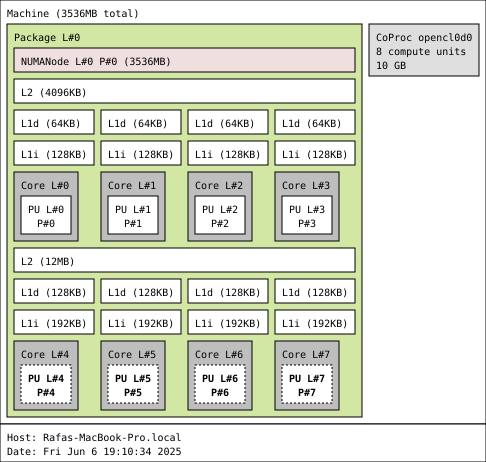
\includegraphics[width=0.8\textwidth]{images/arm.png}
\caption{Topologia procesora Apple M1 z widoczną architekturą big.LITTLE}
\label{fig:m1_topology}
\end{figure}

Platforma ARM64 reprezentowana jest przez komputer Apple MacBook Pro z następującymi specyfikacjami technicznymi:

\begin{table}[h]
\centering
\caption{Specyfikacja platformy ARM64}
\begin{tabular}{|l|l|}
\hline
\textbf{Komponent} & \textbf{Specyfikacja} \\
\hline
Procesor & Apple M1 (ARM64) \\
Architektura & 8 rdzeni (4$\times$P-core + 4$\times$E-core) \\
Pamięć podręczna L2 & 4$\times$12MB (P-cores) + 4$\times$4MB (E-cores) \\
Pamięć operacyjna & 16 GB LPDDR4X unified memory \\
System operacyjny & macOS (Darwin kernel 23.5.0) \\
Jądro systemu & \texttt{arm64} \\
Nazwa hosta & \texttt{mbp-m1} \\
\hline
\end{tabular}

\label{tab:arm64_specs}
\end{table}

Procesor Apple M1 charakteryzuje się architekturą heterogeniczną \eng{big.LITTLE} z rdzeniami o różnej wydajności:
\begin{itemize}
    \item \textbf{Performance cores (P-cores)}: 4 rdzenie wysokowydajne o częstotliwości do 3.2 GHz,
    \item \textbf{Efficiency cores (E-cores)}: 4 rdzenie energooszczędne o częstotliwości do 2.0 GHz,
    \item \textbf{Unified Memory Architecture}: Wspólna pamięć dla CPU i GPU eliminująca kopiowanie danych,
    \item \textbf{Pamięć podręczna}: Hierarchiczna struktura z dedykowanymi poziomami L1/L2 per rdzeń.
\end{itemize}

\subsubsection{Platforma x86\_64 - Intel}
\begin{figure}[H]
\centering
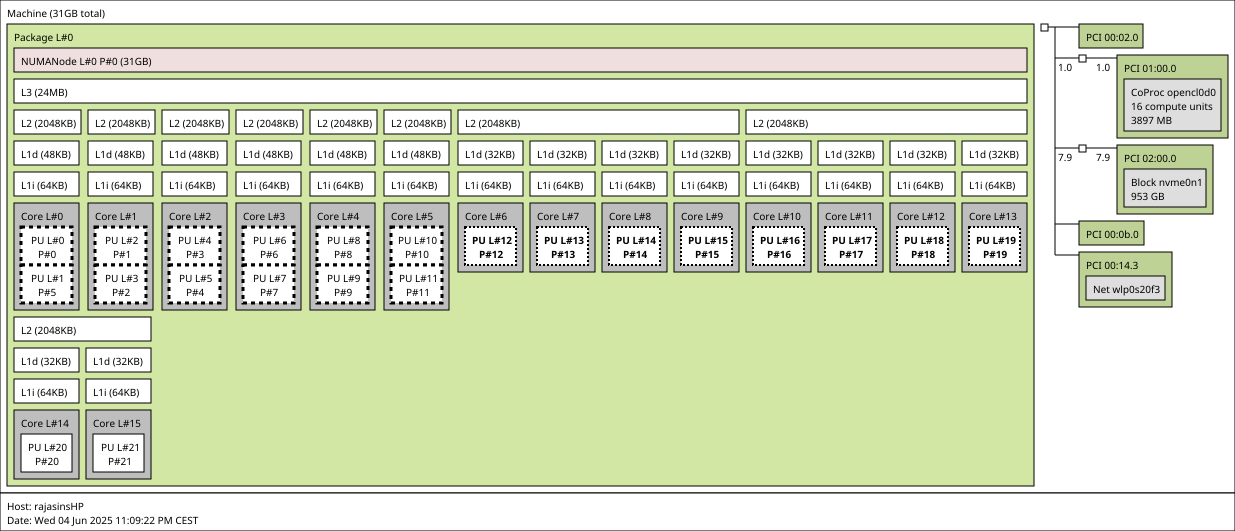
\includegraphics[width=0.8\textwidth]{images/x86.png}
\caption{Topologia procesora Intel Core Ultra 7 165H z widoczną architekturą heterogeniczną}
\label{fig:intel_topology}
\end{figure}
Platforma x86\_64 reprezentowana jest przez komputer HP z następującymi specyfikacjami technicznymi:

\begin{table}[h]
\centering
\caption{Specyfikacja platformy x86\_64}
\begin{tabular}{|l|l|}
\hline
\textbf{Komponent} & \textbf{Specyfikacja} \\
\hline
Procesor & Intel(R) Core(TM) Ultra 7 165H \\
Architektura & x86\_64 (Intel Meteor Lake) \\
Rdzenie całkowite & 22 (16 P-cores + 6 E-cores) \\
Wątki logiczne & 22 (P-cores z Hyper-Threading wyłączonym) \\
Pamięć podręczna L2 & P-cores: 2048KB $\times$ 6, E-cores: 2048KB $\times$ 8 \\
Pamięć podręczna L3 & 24MB współdzielona \\
Pamięć operacyjna & 32 GB DDR5-4800 \\
System operacyjny & Linux Ubuntu 24.04 LTS \\
Jądro systemu & 6.11.0-25-generic \\
Nazwa hosta & \texttt{hp-intel} \\
\hline
\end{tabular}

\label{tab:x86_specs}
\end{table}

Procesor Intel Core Ultra 7 165H (Meteor Lake) również wykorzystuje architekturę heterogeniczną:
\begin{itemize}
    \item \textbf{P-cores}: 6 rdzeni wysokowydajnych z obsługą Hyper-Threading (12 wątków logicznych),
    \item \textbf{E-cores}: 8 rdzeni energooszczędnych (8 wątków logicznych),
    \item \textbf{LP E-cores}: 2 rdzenie niskoenergiczne (2 wątki logiczne),
    \item \textbf{NUMA}: Non-Uniform Memory Access z Package L\#0,
    \item \textbf{Technologie}: Intel Turbo Boost, Intel Speed Shift, Advanced Vector Extensions (AVX2).
\end{itemize}

\subsection{Środowiska programistyczne}

\subsubsection{Kompilatory i narzędzia}

\begin{table}[h]
\centering
\caption{Wersje kompilatorów na platformach testowych}
\begin{tabular}{|l|l|l|}
\hline
\textbf{Platforma} & \textbf{Rust} & \textbf{C++} \\
\hline
ARM64 (macOS) & rustc 1.75.0 & clang++ 14.0.3 \\
x86\_64 (Linux) & rustc 1.75.0 & g++ 11.4.0 \\
\hline
\end{tabular}

\label{tab:compilers}
\end{table}

\subsubsection{Flagi kompilacji}
\begin{itemize}
    \item \textbf{Rust}: \texttt{cargo build --release} z optymalizacjami \texttt{opt-level = 3},
    \item \textbf{C++ (Linux)}: \texttt{g++ -O3 -DNDEBUG -std=c++20 -pthread -march=native},
    \item \textbf{C++ (macOS)}: \texttt{clang++ -O3 -DNDEBUG -std=c++20 -pthread}.
\end{itemize}
\subsection{Narzędzia pomiarowe i diagnostyczne}

\subsubsection{Narzędzia profilowania wydajności}

\subsubsection{Linux x86\_64 - perf}
Monitorowane metryki:
\begin{itemize}
    \item \textbf{Cykle procesora}: Całkowita liczba cykli zegara,
    \item \textbf{Instrukcje}: Liczba wykonanych instrukcji,
    \item \textbf{Cache performance}: Trafienia i chybienia pamięci podręcznej,
    \item \textbf{Predykcja rozgałęzień}: Dokładność mechanizmów przewidywania rozgałęzień warunkowych,
    \item \textbf{Przełączenia kontekstu}: Liczba operacji zmiany kontekstu wykonywania.
\end{itemize}

\subsubsection{macOS ARM64 - Instruments}
Wykorzystanie pakietu Xcode Instruments:
\begin{itemize}
    \item \textbf{System Trace}: Analiza planowania wątków i synchronizacji,
    \item \textbf{Allocations}: Monitorowanie alokacji i dealokacji pamięci,
    \item \textbf{Time Profiler}: Profilowanie czasowe z dokładnością do funkcji,
    \item \textbf{System Usage}: Wykorzystanie zasobów systemowych.
\end{itemize}